\documentclass[a4paper, 12pt]{article}
\usepackage{graphicx} % Required for inserting images
\usepackage{titling}
\usepackage{algorithm}
\usepackage[english]{babel}
\usepackage{algpseudocode}
\usepackage{amsmath}
\usepackage{amsfonts} 
\usepackage{natbib}
\bibliographystyle{plain}

\title{S1 Statistical Methods - Coursework \\ Multi-Dimensional Probability Distribution}
\author{Zihan Xu (zx282)}
\date{Michaelmas Term 2024}


\begin{document}
\maketitle
\begin{center}
    Word Count: 2131
\end{center}

\section{Introduction}
\hspace{1.5em}This report discusses statistical methods in estimating parameters for a particular target distribution, with its definition outlined in the next two sections. 
\section{Normalisation Constant}
\hspace{1.5em}To compute the normalization constant, we use the fundamental property that a probability density function must integrate to unity over its domain:
\begin{equation}
    \int_{-\infty}^{\infty} \rho (X;\mu,\sigma,\beta, m) dx = 1
\end{equation}
\par Using a change of variable $Z = \frac{x-\mu}{\sigma}$, $\sigma dz = dx$. Plug this and the full expression of the probability density function into equation (1):
\\
\begin{equation*}
    \sigma N (\int_{-\beta}^{\infty} e^{-z^{2}/2}dz + \int_{-\infty}^{-\beta}(\frac{m}{\beta})^{m}e^{-\beta^{2}/2} (\frac{m}{\beta} - \beta - z)^{-m} dz) = 1
\end{equation*}
\par Note that the first term, the Gaussain integral, is an even function. By exploitting this symmetry, the limits of the integral could be flipped: 

\begin{align*}
    N^{-1} &= \sigma \left( \int_{-\infty}^{\beta} e^{-\frac{z^2}{2}} \, dz 
    + e^{-\frac{\beta^2}{2}} \left( \frac{m}{\beta} \right)^m 
    \int_{-\infty}^{-\beta} \left( \frac{m}{\beta} - \beta - z \right)^{-m} \, dz \right) \\
    &= \sigma \left( \sqrt{2\pi} \Phi(\beta) + e^{-\frac{\beta^2}{2}} 
    \left( \frac{m}{\beta} \right)^m 
    \left[ -\frac{\left( \frac{m}{\beta} - \beta - z \right)^{-m+1}}{-m + 1} \right]_{z=-\infty}^{z=-\beta} \right) \\
    &= \sigma \left( \sqrt{2\pi} \Phi(\beta) + e^{-\frac{\beta^2}{2}} 
    \left( \frac{m}{\beta} \right)^m \left( \frac{m}{\beta} \right)^{1-m} \frac{1}{m-1} \right) \\
    &= \sigma \left( \sqrt{2\pi} \Phi(\beta) + \frac{m}{\beta (m-1)} e^{-\frac{\beta^2}{2}} \right)
\end{align*}
which yields the desired result. 


\section{The Statistical Model}
\hspace{1.5em}From the description of the model, the following expression could be derived for the signal and background distributions:
The signal probability distribution: 
\begin{equation*}
    f_{s}(X,Y) = N_{s} * \begin{cases}
\lambda e^{-Z^2/2} e^{-\lambda Y} & Z \geq -\beta \\
(\frac{m}{\beta})^{m} e^{-\beta^{2}/2}(\frac{m}{\beta} -\beta - Z)^{-m} & Z \leq -\beta 
\end{cases}
\end{equation*}
where $N_{s}$ is identical to the one derived in the previous section and $\beta, \lambda > 0$, $m > 1$ and $Z = (X-\mu)/\sigma$, $\sigma > 0$. \par 
The background distribution:
\begin{equation*}
   f_{b}(X,Y) = N_{b} \frac{1}{5\sigma_{b}\sqrt{2\pi}} e^{-\frac{1}{2}(\frac{x-\mu_{b}}{\sigma_{b}})^2}
\end{equation*}
where $\sigma_{b}>0$. 
\par For both $f_{s}(X,Y)$ and $f_{b}(X,Y)$, the definition above is valid for $X \in [0,5], Y \in [0,10]$. Beyond these intervals, $f_{s}(X,Y) = f_{b}(X,Y) = 0$. 
\par $N_{s}$ and $N_{b}$ are normalizing constants. The normalization constants $N_s$ and $N_b$ must be computed separately due to their different analytical properties:\par
- $N_b$ can be calculated directly using the cumulative distribution function via \texttt{stats.norm.cdf} since cumulative distribution function for $f_{b}$ is known. \par
- $N_s$ requires numerical integration using \texttt{scipy.integrate.quad} as it lacks an analytical solution. The inverse of the numerical integration results give rise to value for $N_s$.
\par 
The complete model combines these distributions:
\begin{equation}
    f(x,y) = f f_s(x,y) + (1-f) f_b(x,y)
\end{equation}

The full implementation is available in \texttt{code/total\_model.py}.


\section{Probability Density Function Visualisation}
\hspace{1.5em}To visualize the probability density function $f(x,y)$, we generate both marginal projections and a two-dimensional density plot. The visualization process involves: \par 
1. Discretisation: The function input is sampled on a uniform grid of $500 \times 500$ points covering the domain $[0,5] \times [0,10]$\par
2. Projections: The marginal distributions is computed by integrating over each variable:
   
   \begin{align}
   f_X(x) &= \int_0^{10} f(x,y) \, dy \\
   f_Y(y) &= \int_0^5 f(x,y) \, dx
   \end{align}
\par 
3. Two-dimensional visualization: the full joint density $f(x,y)$ is plotted as a heat-map over the rectangular domain. \par 
The complete implementation of these visualizations can be found in \texttt{code/total\_model.py}.
\begin{figure}[H]
    \centering
    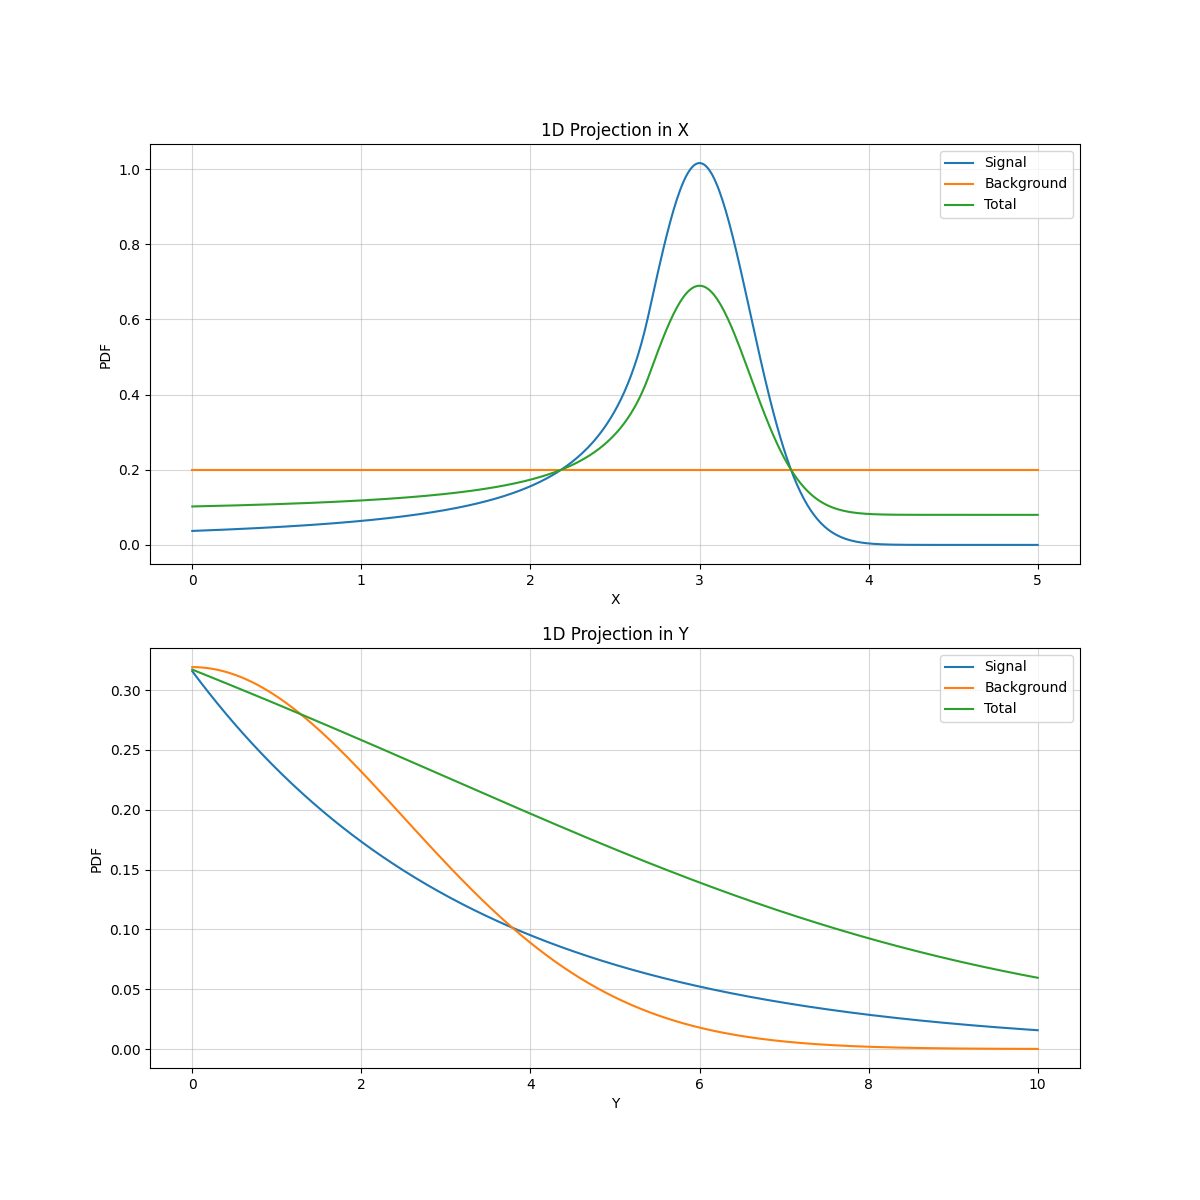
\includegraphics[height=12cm]{plots/q3_1d_projection.png}
    \caption{Marginal distributions of the model}
    \label{fig:marginal_distributions}
\end{figure}
\par Here, all the distributions are normalized accordingly, which allows for direct comparison of their shapes and relative contributions. In the $x$-projection, the signal distribution shows a clear peaked structure centered at $x=3$, with a relatively narrow width, suggesting a well-defined signal region. The peak reaches a maximum PDF value of approximately $1.0$, where the signal is most concentrated. The tails of the signal distribution fall off quickly on both sides, suggesting good signal containment in this variable. The signal stands out clearly against the flat background, which has constant value of $0.2$. The uniform background component imposed a broadening effect on the sharply peaked signal distribution, resulting in a more diffuse total distribution, which is obtained by taking weighted sum of signal and background. The three curves crosses twice, with the first time around $x=2.1$ and the second time near $x=3.6$, where they share the same value of $0.2$. 
\par In the $y$-projection, the distinct curvature of background and signal yields a flatter total model. The background shows a steep exponential-like decay from its initial value at y=0, while the signal exhibits a more gradual decrease with a long tail extending to higher $y$ values. These different shapes result in a total distribution that follows an intermediate trajectory, with crossing points near y=4 where the signal-to-background ratio changes significantly. 
\begin{figure}[H]
    \centering
    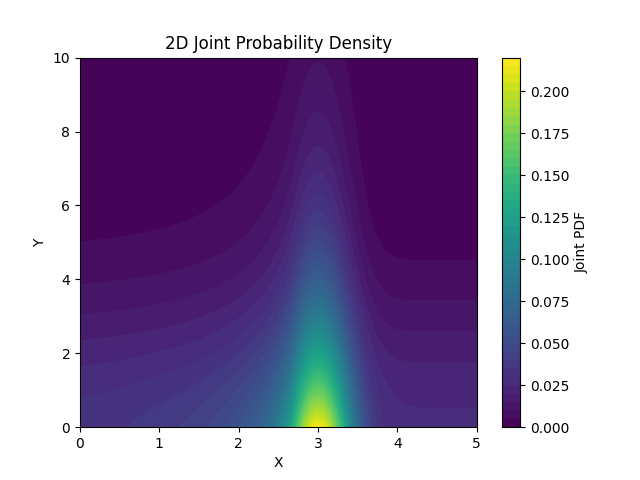
\includegraphics[height=12cm]{plots/q3_2d_plot.png}
    \caption{Joint distributions of the model}
    \label{fig:marginal_distributions}
\end{figure}
\par The joint probability density function shows a region of high density along $x = 3$. The global maximum of the distribution occur at the point $(x,y) = (3,0)$. This feature emerges from the mixture between the Gaussian nature of the background distribution centered at $x = 3$ and the exponential decay of the signal component in the y-direction. The color gradient in the plot ranges from dark purple (low density) to bright yellow (high density),which illustrates the concentration of probability mass. Moving away from $x = 3$ in either direction, the density falls off symmetrically, which is consistent with the Gaussian behavior observed in the x-projection. 
\par This 2D representation reveals the full structure of the correlation between x and y variables. The graph also visualizes the different scales of variation in the x and y directions. The x-direction shows a relatively compact distribution within the region$x \in [2,4]$, while the y-direction demonstrates significant probability density extending beyond $y > 4$. This behavior is consistent with the longer tails observed in the y-projection plot. 
\section{Extended Maximum Likelihood Estimation of Parameters}
\hspace{1.5em}The joint distribution presents a challenge for the generation of samples because its cumulative distribution function has no closed analytical form. The accept-reject sampling method offers a solution to this limitation. This technique is particularly valuable because it enables direct sampling from the probability density function without requiring knowledge of the cumulative distribution function \cite{lecturenotes2024}. 
\par However, the efficiency of the accept-reject method is suboptimal. The implementation adopts vectorized operations to enhance performance. Multiple candidate samples are generated simultaneously for the accept-reject criterion, using \textit{numpy}'s efficient vector computations to accelerate the sampling process. The implementation is presented in \textit{code/generate$\_$sample.py}.
\par Maximum likelihood estimation of the $9$ parameters,  $N$, $\mu$, $\sigma$, $\beta$, $m$, $f$, $\lambda$, $\mu_{b}$ and $\sigma_{b}$ is performed using the package \textit{Minuit}. The starting value used for \textit{Minuit} is $\mu = 0,\sigma = 1, \beta = 1,m = 1,f = 0.5,\lambda = 0.1,\mu_b = 0.5,\sigma_b = 1$. These initial values are selected to be in proximity to the true parameter values to demonstrate the effectiveness of the maximum likelihood estimation method. To enhance computational efficiency and ensure convergence, bounds are implemented for each parameter during the optimization process. 
\par The estimated parameter value and error are the following:
\begin{table}[H]
\centering
\begin{tabular}{|c|ccccc|} \hline
Parameter & $N$           & $\mu$   & $\sigma$ & $\beta$    & $m$    \\ \hline
Value     & 100000.1158 & 2.9998  & 0.2986   & 1.0033     & 1.4008 \\
Error     & 316.2279    & 0.0026  & 0.0024   & 0.0219     & 0.0612 \\ \hline
Parameter & $f$           & $\lambda$ & $\mu_{b}$  & $\sigma_{b}$ &        \\
Value     & 0.6016      & 0.3006  & 0.1079   & 2.4253     &        \\
Error     & 0.0035      & 0.0020  & 0.0733   & 0.0351     &        \\ \hline
\end{tabular}
\caption{Extended Maximum Likelihood Estimation Result}
\end{table}
\par 
The parameters $\mu$ and $\sigma$ both demonstrate remarkably small relative errors of about $0.087\%$ and $0.80\%$ respectively, indicating high precision in these estimates. Similarly, $\beta$ and $m$ show modest relative errors of $2.18\%$ and $4.37\%$, respectively. In the second set of parameters, $f$ and $\lambda$ maintain this pattern of precision with relative errors of $0.58\%$ and $0.67\%$ respectively. However, $\mu_{b}$ shows a larger relative error of about $67.9\%$, suggesting that this parameter estimate is less reliable. Finally, $\sigma_{b}$ has a relatively small error of $1.45\%$ compared to its value. In general, there is a small relative errors across most parameters, suggesting the estimation method was quite effective.
\\
\par The execution time of generating the samples and the maximum likelihood fit are presented relative to the execution time of generating normal distribution samples. The figures are the following:
\par - Generating joint distribution sample / Generating normal sample: $56.94$
\par - Parameter Estimation / Generating normal sample: $4048.09$ 
\par These figures are calculated by taking the mean over 100 executions. The substantial computational time in joint distribution generation is attributed to the implementation of the accept-reject sampling method, which is known for its lower efficiency. The considerable computational cost from parameter estimation fit originates from the optimization algorithms involving multiple iterations of likelihood evaluations across the nine-dimensional parameter space.
\par All the implementation are recorded in \textit{code/generate$\_$sample.py}. The time of the execution is recorded using the \textit{timeit} python library. 
\section{Parametric Bootstrapping}
\hspace{1.5em}The impact of sample size on parameter estimation accuracy was investigated through a comprehensive parametric bootstrapping study, implemented in \textit{code/bootstrap.py}. For each sample size in the analysis, $250$ independent experiments were conducted to obtain statistically meaningful results. This systematic approach allows quantification of both the bias and expected uncertainty in the parameter estimates as functions of sample size. The following figure illustrates these relationships for the background rate parameter $\lambda$:
\begin{figure}[H]
    \centering
    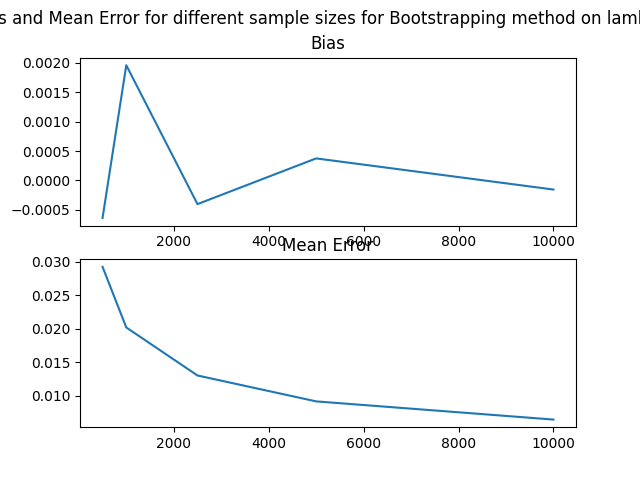
\includegraphics[height = 10cm]{plots/e_bootstrape_plot.png}
    \caption{Bias and Mean Error as Function of Sample Sizes}
    \label{fig:enter-label}
\end{figure}
\par The bootstrap analysis reveals two key patterns in the estimation of $\lambda$. The bias shows a complex behavior: it starts at approximately $0.008$ for small sample sizes, then rapidly decreases to around $0.005$ at $n=2000$. It then exhibits some fluctuation before reaching a minimum of about $0.004$ around $n=5000$. Beyond this point, there's a slight upward trend in bias as the sample size increases to $10000$, suggesting that larger samples may not necessarily lead to better bias reduction in this case.

\par The mean error continues to decrease with increasing sample size, following the expected behavior of maximum likelihood estimation. It is showing an exponential decay from about $0.03$ at small sample sizes to approximately $0.003$ at $n=10000$. This decline is particularly steep until $n=2000$, after which it continues decreases with a more gradual rate. This indicates that additional data improves estimation precision.

\section{sWeights}
\hspace{1.5em}The samples generated through parametric bootstrapping are saved as $npz$ files and used for parameter estimation using sWeights. These sWeights method project out the signal density in the Y variable, which is then used for parameter estimation through maximum likelihood methods. This parameter estimation approach is inspired the capabilities of \textit{iminuit} in estimating parameters in high-dimensional space. By obtaining sWeights in the X variable, weighted maximum likelihood estimation can be performed over y coordinate. This is likely to result in improved prediction of both signal and background components in the Y variable, yielding more accurate parameter estimates. To demonstrate such behavior, prediction of the $\lambda$ parameter, which controls the shape of signal in $y$ coordinate, is conducted. 
\par The implementation of this method is inside \textit{code/sweight$\_$projection.py}, which follows instruction from tutorial notebook from the sWeights package \cite{sweights_docs}. The bias and uncertainty of estimation for $\lambda$ is produced using the script \textit{code/analyze$\_$efg.py} and presented below:
\begin{figure}[H]
    \centering
    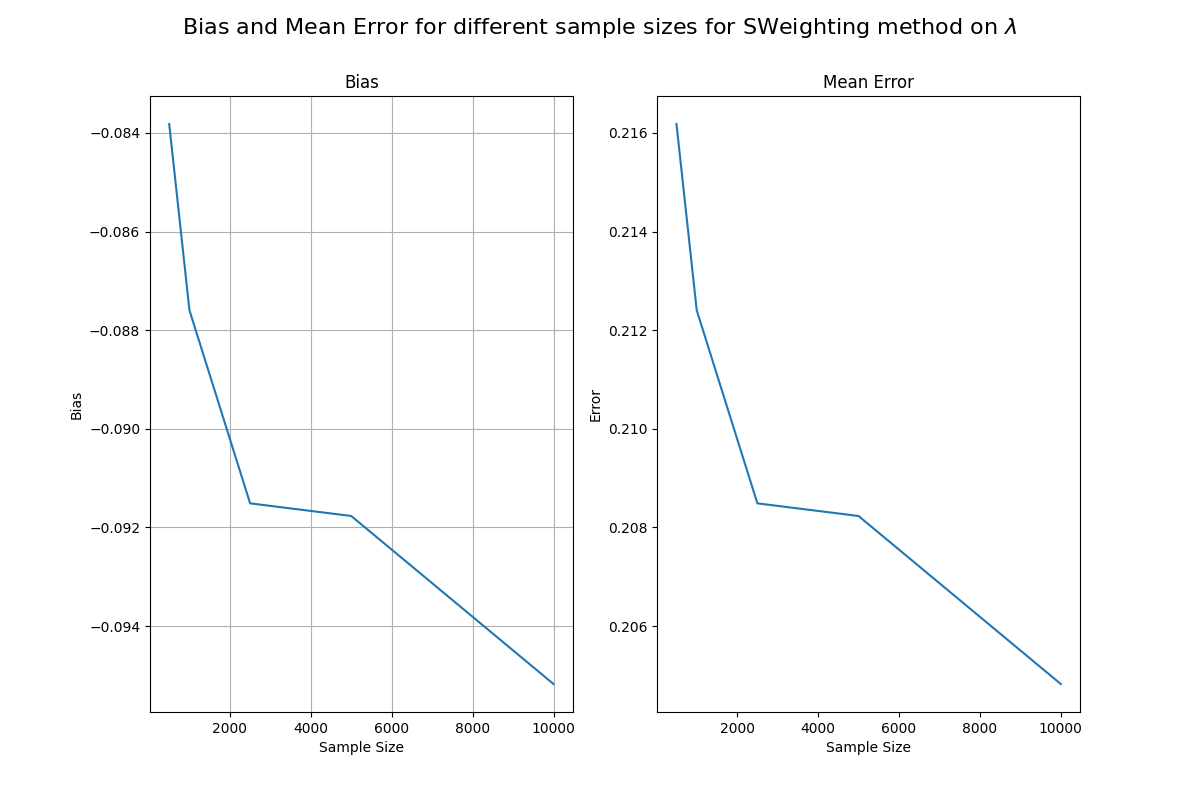
\includegraphics[height = 10cm]{plots/f_sweight_plot.png}
    \caption{Bias and Mean Error for $\lambda$ as Function of Sample Sizes with sWeights}
    \label{fig:enter-label}
\end{figure} 
\par The bias and mean error exhibit almost identical shapes, with both metrics showing an overall downward trend as sample size increases. Both metrics came to a turning point as sample size increases up to $n=5000$. Beyond this point, the metrics simultaneously increases mildly. This unexpected behavior suggests that larger sample sizes do not necessarily guarantee better performance when using sWeights and maximisation of likelihood function for parameter estimation.
\par Notably, the bootstrapping method produces similar bias values compared to the sWeight approach. Although the sWeight method imposes a restrictive assumption that background and signal components follow identical distributions in both $X$ and $Y$ coordinates, it incorporates the predicted function's shape into the estimation process. This additional shape information appears to counterbalance the bias introduced by the distributional assumption.
\par The bootstrapping and sWeight methods demonstrate different behaviors in their mean error performance. The bootstrapping method follows expected theoretical principles, with mean error decreasing as sample size grows. In contrast, the sWeight method deviates from such principle. Additionally, the sWeight method produces larger mean errors compared to bootstrapping, suggesting that bootstrapping provides more reliable parameter estimates for this probability distribution. However, the current analysis of sWeight's performance is limited by its reliance on maximum likelihood estimation. A more comprehensive evaluation would require investigating alternative estimation methods, which might yield different results for the sWeight approach.

\section{Comparative Analysis of Bootstrapping and sWeight Methods}
\hspace{1.5em}To better analyze the performance of sWeight methods against bootstrapping, the bias and mean error for both methods are plotted on the same graph:
\begin{figure}[H]
    \centering
    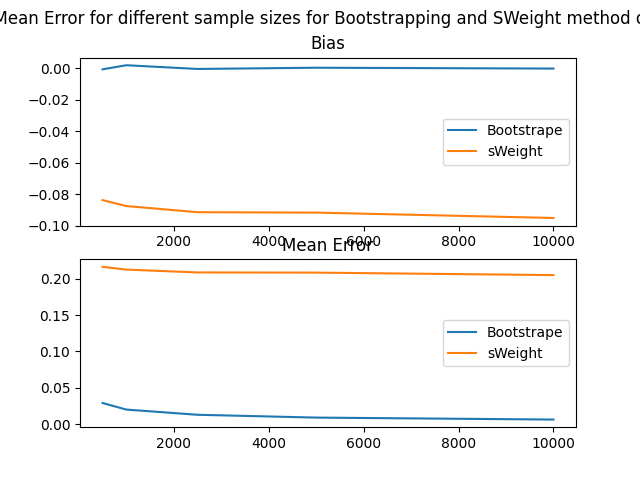
\includegraphics[height = 8cm]{plots/g_comparison_plot.png}
    \caption{Bias and Mean Error for Bootstrapping and sWeight Method}
    \label{fig:enter-label}
\end{figure}
\par The bootstrap method demonstrated superior performance, yielding similar bias but significantly lower mean error compared to sWeight approach. While these results are promising, the evaluation of the sWeight method remains incomplete. The current analysis relied on a single parameter estimation technique, limiting the understanding of its full capabilities. Future research should explore diverse estimation methods to comprehensively assess sWeight's effectiveness in parameter estimation across different scenarios and conditions.
\par Parametric bootstrapping provides a straightforward implementation with fewer statistical assumptions compared to the sWeight method. However, its reliance on repeated sampling from the target distribution makes it computationally expensive. In contrast, the sWeight method employs extended maximum likelihood estimation, requiring deeper statistical expertise but offering greater computational efficiency once the weights are established. The graph demonstrates that sWeights achieves superior classification accuracy with minimal training data, indicating its computational efficiency. 
\par From a statistical perspective, parametric bootstrapping quantifies both bias and mean error without requiring a perfectly specified model. This makes it particularly valuable when large sample sizes are available but distributional assumptions are limited. The sWeight method, however, requires well-defined background and signal models, enabling efficient estimation with substantially lower computational resource demands. 
\par These methodological differences suggest distinct use cases. The sWeights method generally is more appropriate in cases where signal and background shapes are well-understood from theory or simulation in at least one dimension \cite{sweights2020}, while computing resources need careful management, and complex correlations between variables must be handled in large datasets. Parametric bootstrapping can be computationally demanding for large datasets and may struggle with complex correlations, while showing sensitivity to parameter choice and requiring careful validation of the bootstrap procedure. This method could be used as a starting point in forming hypothesis for behavior of the dataset. 
\par Note that these methods are not mutual exclusive. They can serve complementary effects and perform validation for one another. The ultimate choice between methods should consider the specific analysis requirements, available computing resources, understanding of signal and background models, and the relative importance of robust uncertainty estimation versus statistical efficiency.



\section{Acknowledgment}
\hspace{1.5em}This report was developed with the assistance from Anthropic's Claude 3.5 Sonnet. Specifically, Claude was used to improve the clarity of written content and assist with debugging Python code implementations of statistical analysis methods. All AI-generated suggestions were manually reviewed. 

\newpage
\bibliography{references}

\end{document}
